\chapter{Project Specification}
Summary of the project outline.

\section{Functional Requirements}
some text here

\section{Non-Functional Requirements}
some text here

\chapter{Project Management}
Discussion on how the project was managed. What things impacted the success of the project. How does the continually revised versions of the project plan compare to the initial draft developed at the start of the project. Did everything run according the schedule. Did elements such as exams \& coursework have any impact. 

\chapter{Implementation Appendix}

\begin{figure}[!htbp]
    \centering
    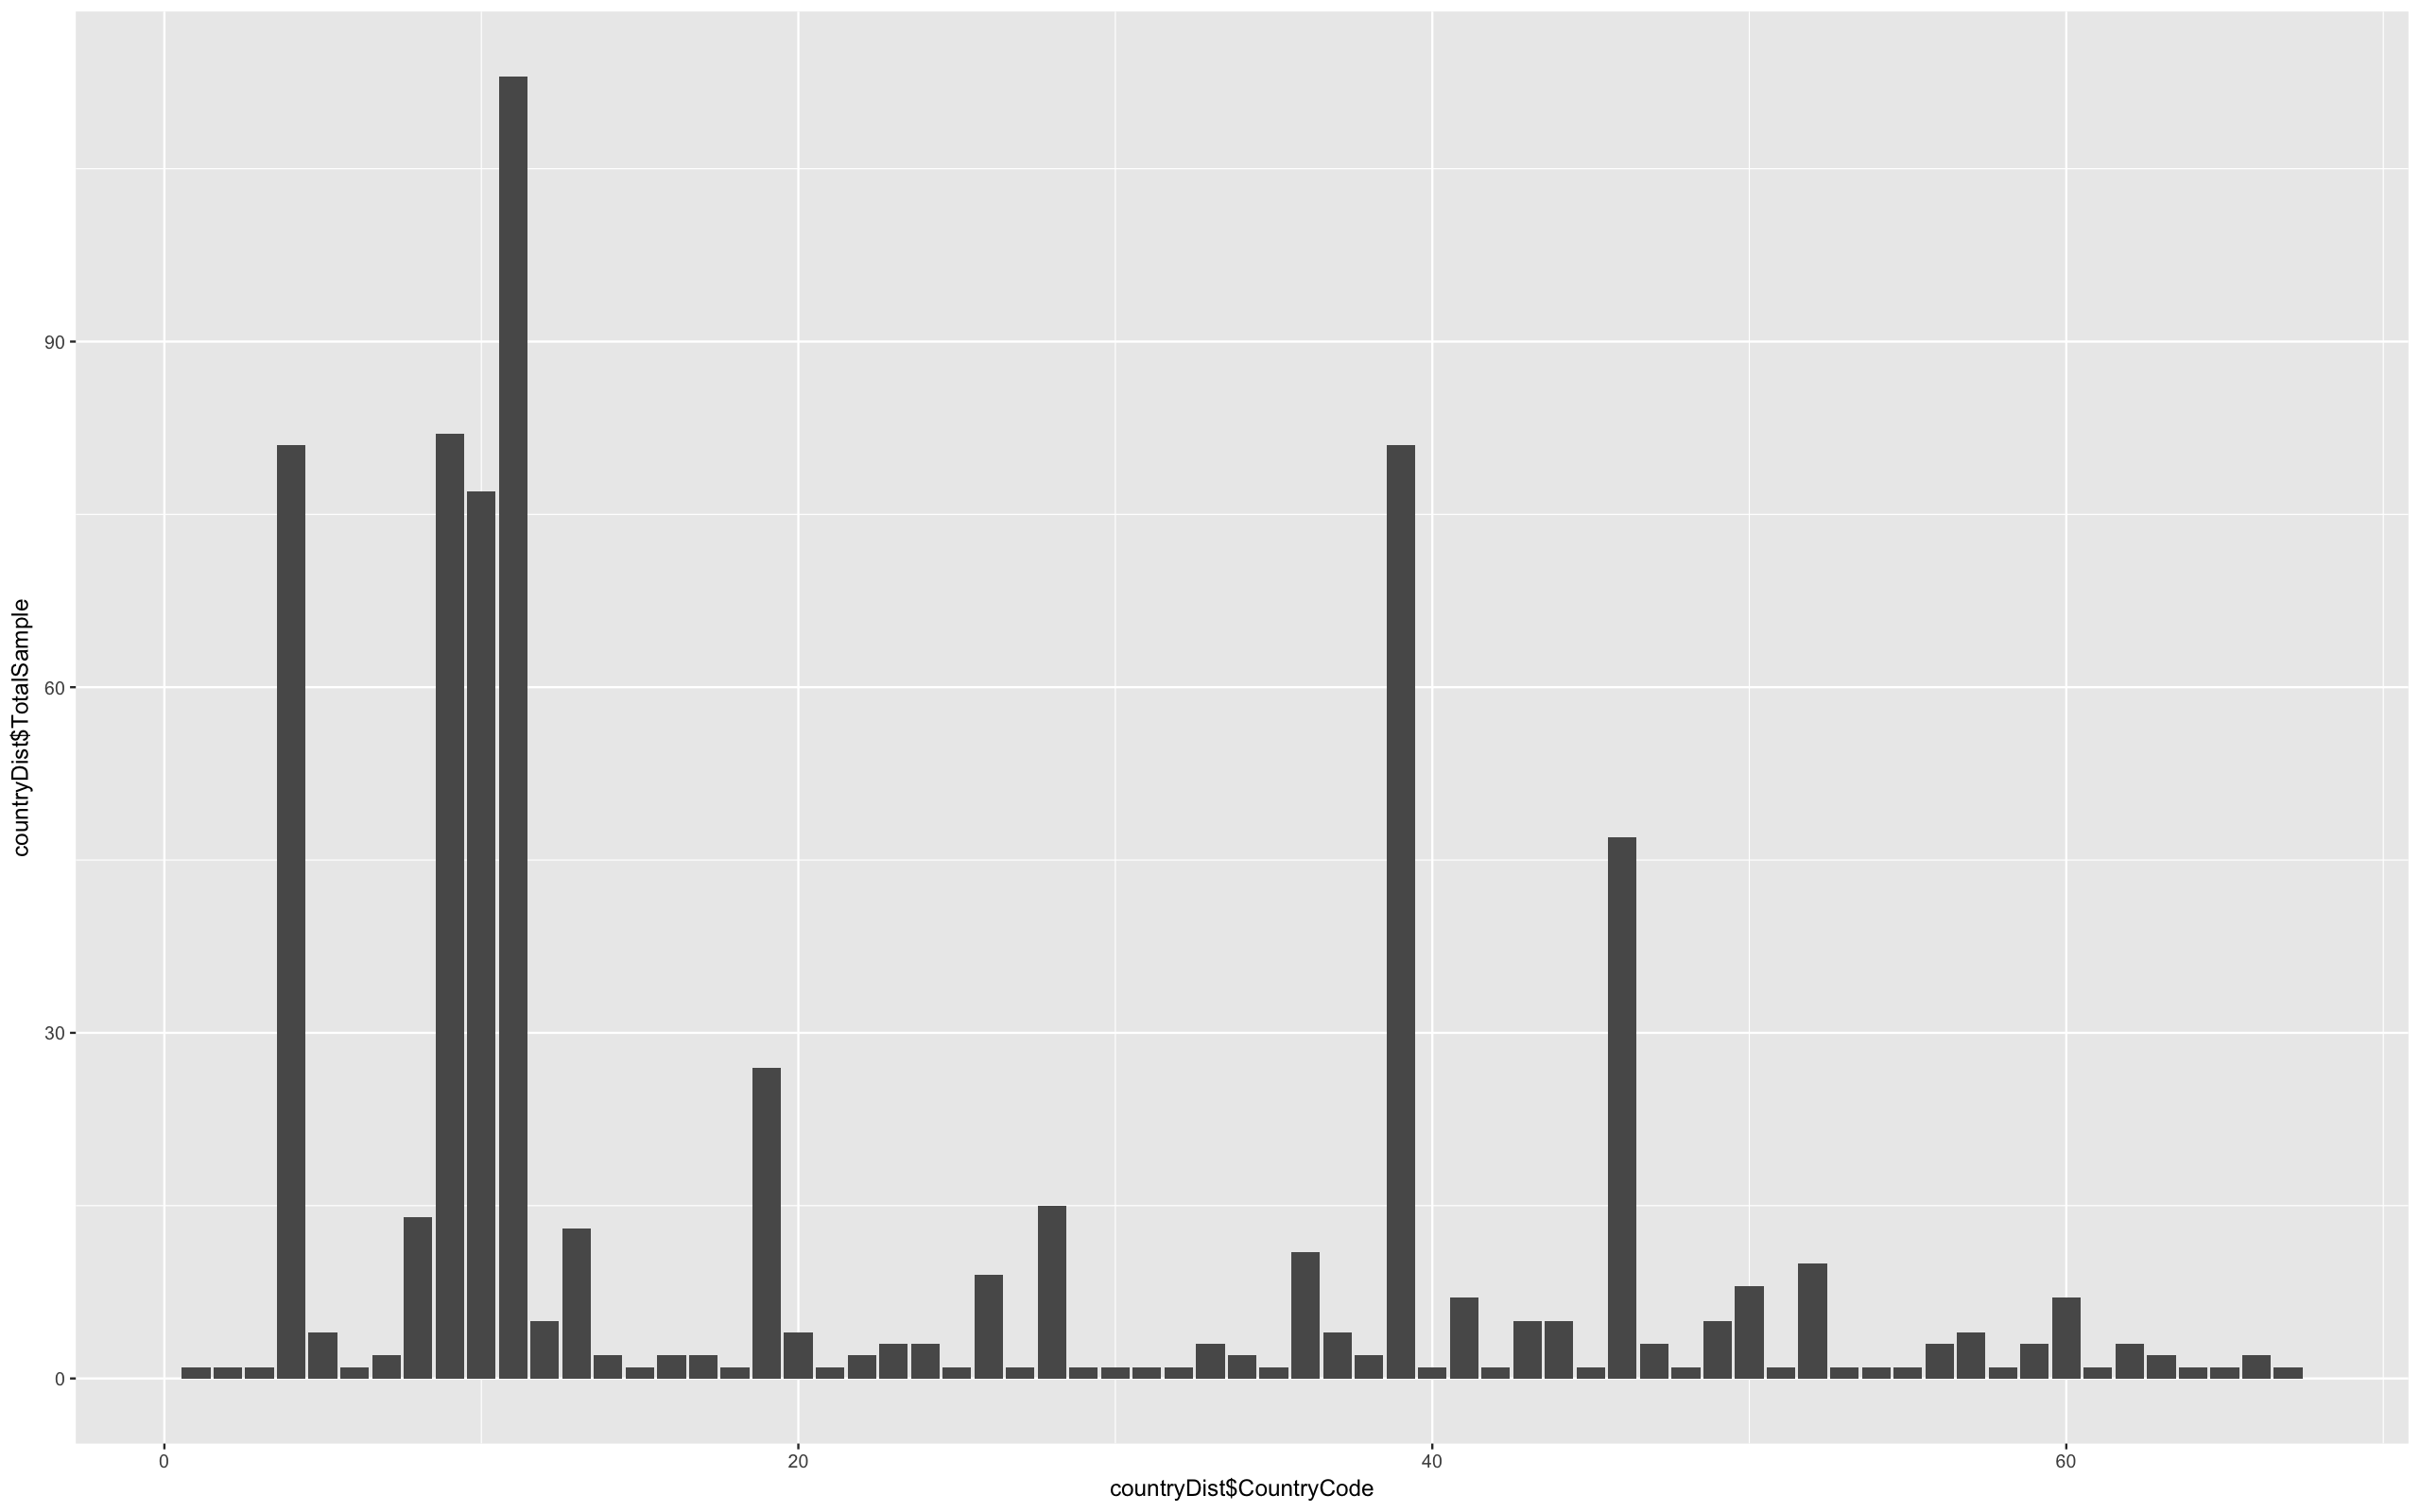
\includegraphics[width=0.9\textwidth]{ThesisTemplate/appendix/images/figure4_2b.png}
    \caption{Distribution of the autism data by country of residence.}
    \label{fig:my_label}
\end{figure}

\chapter{Evaluation Appendix}
\begin{figure}[!htbp]
    \centering
    \begin{minipage}{0.45\textwidth}
        \centering
        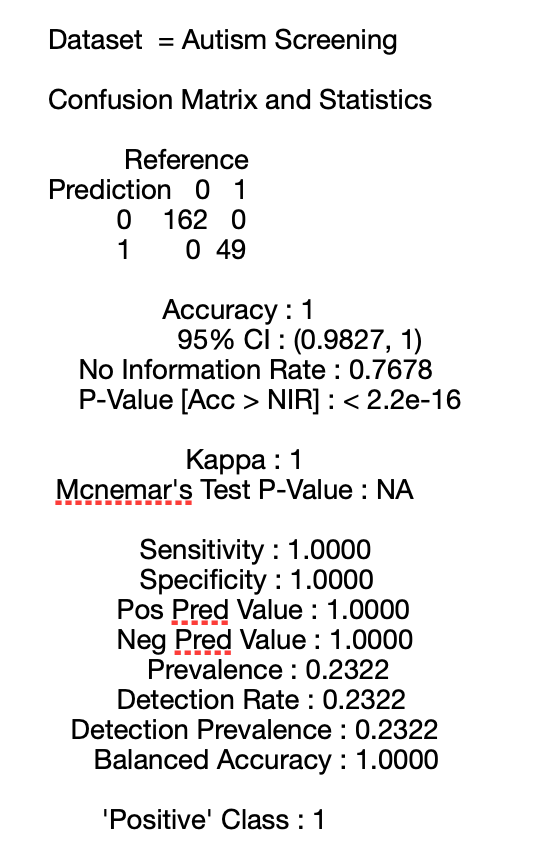
\includegraphics[width=0.9\textwidth]{ThesisTemplate/appendix/images/Chapter5Appendix/ConfusionMatrix/Autism.png} 
        \caption{Confusion Matrix output for Random Forest fitted to the Autism Dataset}
        \label{fig:my_label}
    \end{minipage}\hfill
    \begin{minipage}{0.45\textwidth}
        \centering
        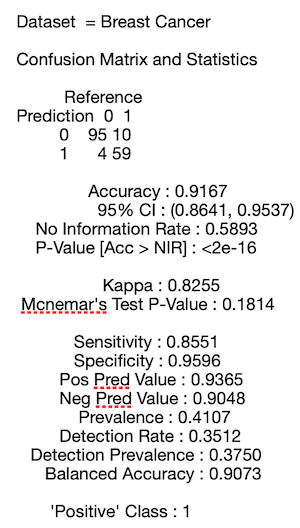
\includegraphics[width=0.9\textwidth]{ThesisTemplate/appendix/images/Chapter5Appendix/ConfusionMatrix/BreastCancer.png} 
        \caption{Confusion Matrix output for Random Forest fitted to the Breast Cancer Dataset}
        \label{fig:my_label}
    \end{minipage}
\end{figure}

\begin{figure}[!htbp]
    \centering
    \begin{minipage}{0.45\textwidth}
        \centering
        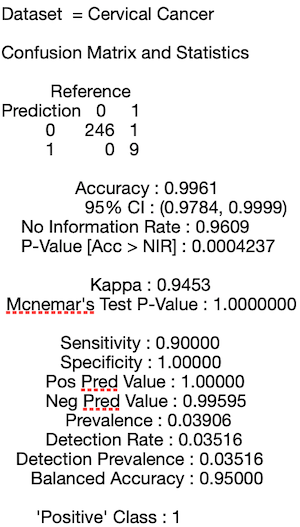
\includegraphics[width=0.9\textwidth]{ThesisTemplate/appendix/images/Chapter5Appendix/ConfusionMatrix/CervicalCancer.png} 
        \caption{Confusion Matrix output for Random Forest fitted to the Cervical Cancer Dataset}
        \label{fig:my_label}
    \end{minipage}\hfill
    \begin{minipage}{0.45\textwidth}
        \centering
        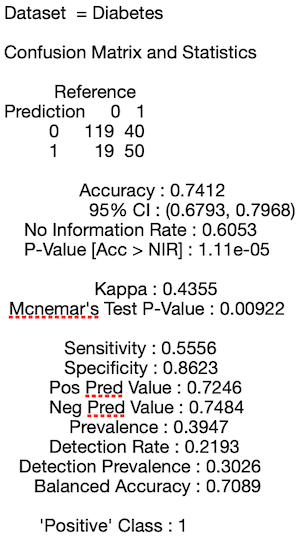
\includegraphics[width=0.9\textwidth]{ThesisTemplate/appendix/images/Chapter5Appendix/ConfusionMatrix/Diabetes.png} 
        \caption{Confusion Matrix output for Random Forest fitted to the Diabetes Dataset}
        \label{fig:my_label}
    \end{minipage}
\end{figure}

\begin{figure}[!htbp]
    \centering
    \begin{minipage}{0.45\textwidth}
        \centering
        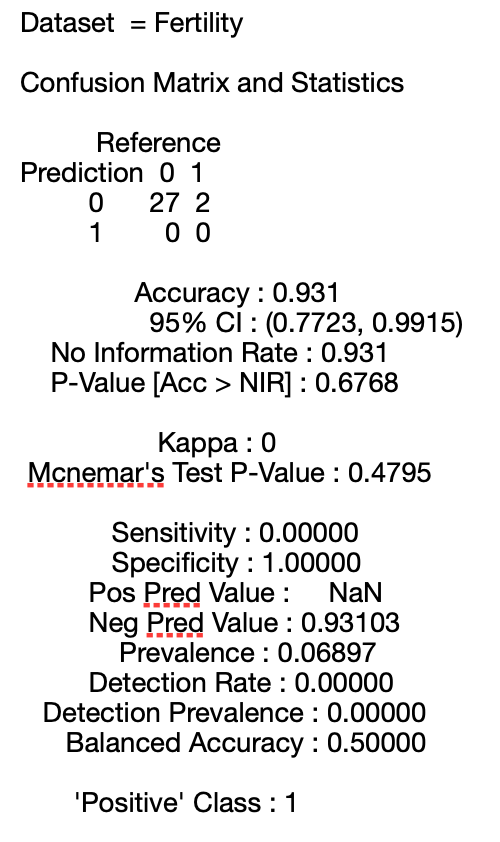
\includegraphics[width=0.9\textwidth]{ThesisTemplate/appendix/images/Chapter5Appendix/ConfusionMatrix/Fertility.png} 
        \caption{Confusion Matrix output for Random Forest fitted to the Fertility Dataset}
        \label{fig:my_label}
    \end{minipage}\hfill
    \begin{minipage}{0.45\textwidth}
        \centering
        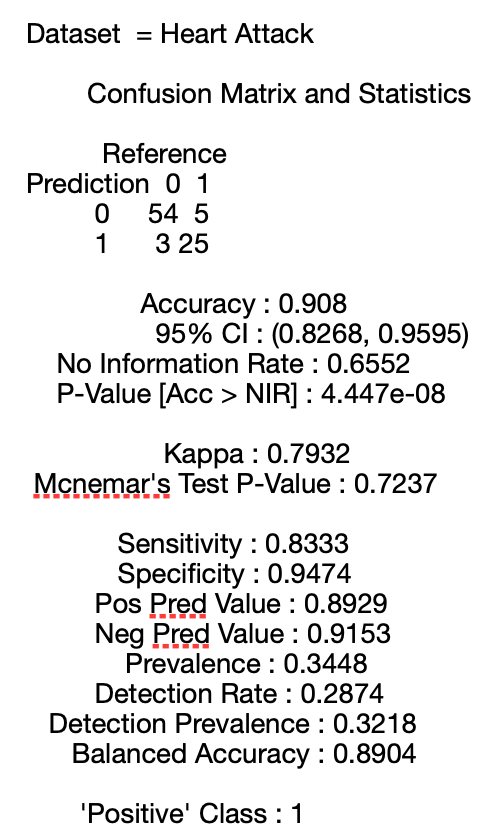
\includegraphics[width=0.9\textwidth]{ThesisTemplate/appendix/images/Chapter5Appendix/ConfusionMatrix/HeartAttack.png} 
        \caption{Confusion Matrix output for Random Forest fitted to the Heart Attack Dataset}
        \label{fig:my_label}
    \end{minipage}
\end{figure}


\begin{figure}[!htbp]
    \centering
    \begin{minipage}{0.45\textwidth}
        \centering
        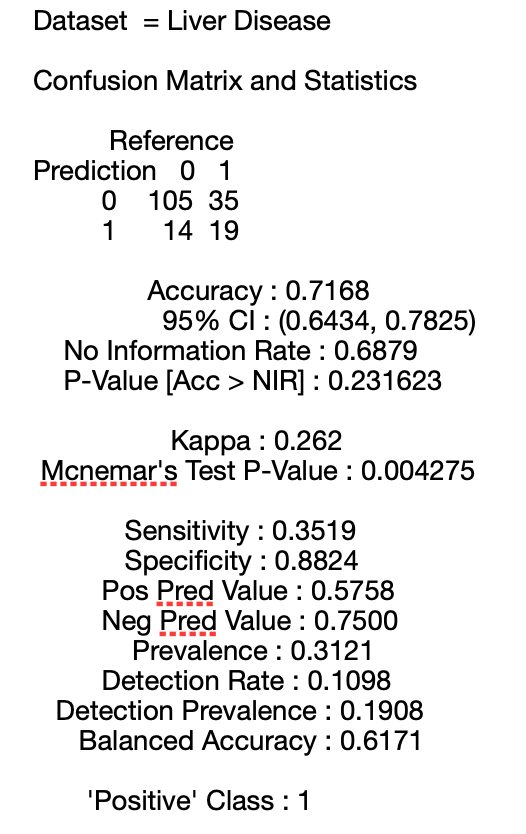
\includegraphics[width=0.9\textwidth]{ThesisTemplate/appendix/images/Chapter5Appendix/ConfusionMatrix/LiverDisease.png} 
        \caption{Confusion Matrix output for Random Forest fitted to the Liver Dataset}
        \label{fig:my_label}
    \end{minipage}\hfill
    \begin{minipage}{0.45\textwidth}
        \centering
        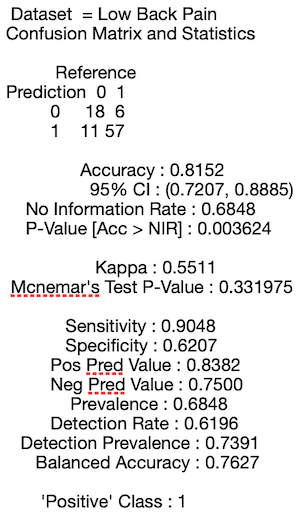
\includegraphics[width=0.9\textwidth]{ThesisTemplate/appendix/images/Chapter5Appendix/ConfusionMatrix/LowBackPain.png} 
        \caption{Confusion Matrix output for Random Forest fitted to the Low Back Pain Dataset}
        \label{fig:my_label}
    \end{minipage}
\end{figure}

\begin{figure}[!htbp]
    \centering
    \begin{minipage}{0.45\textwidth}
        \centering
        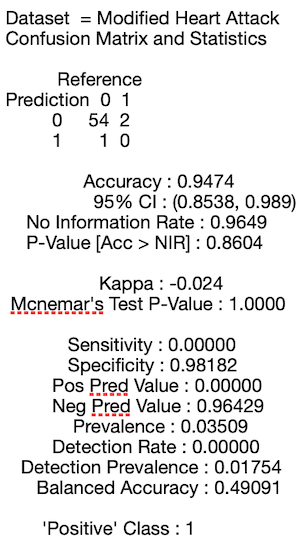
\includegraphics[width=0.9\textwidth]{ThesisTemplate/appendix/images/Chapter5Appendix/ConfusionMatrix/modHeartAttack.png} 
        \caption{Confusion Matrix output for Random Forest fitted to the Modified Heart Attack Dataset}
        \label{fig:my_label}
    \end{minipage}\hfill
    \begin{minipage}{0.45\textwidth}
        \centering
        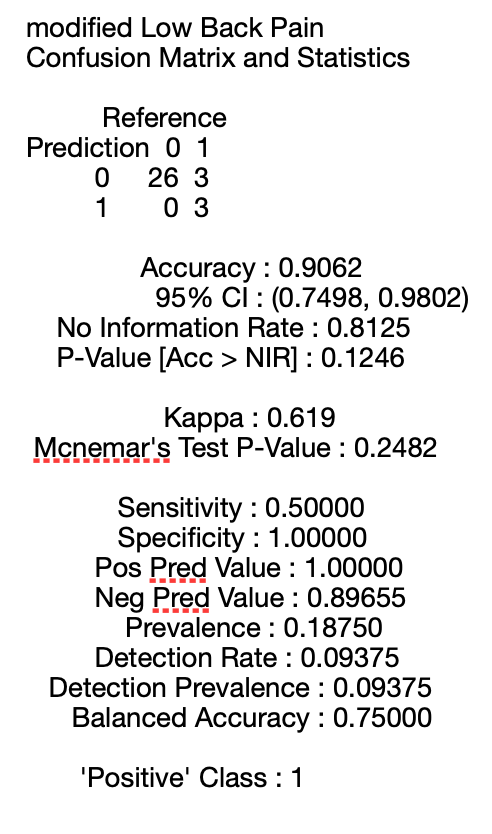
\includegraphics[width=0.9\textwidth]{ThesisTemplate/appendix/images/Chapter5Appendix/ConfusionMatrix/modLowBackPain.png} 
        \caption{Confusion Matrix output for Random Forest fitted to the Modified Low Back Pain Dataset}
        \label{fig:my_label}
    \end{minipage}
\end{figure}


\begin{figure}[!htbp]
    \centering
    \begin{minipage}{0.45\textwidth}
        \centering
        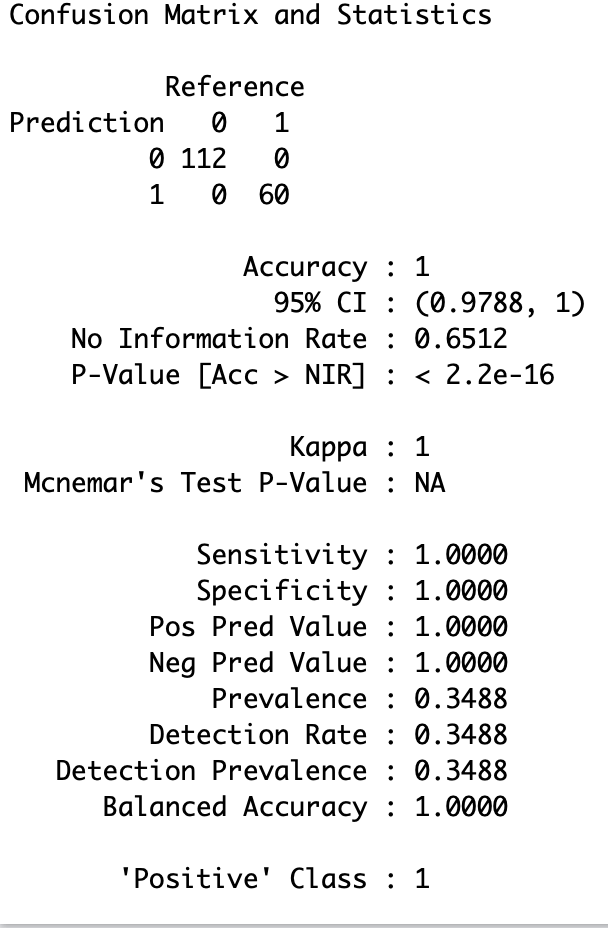
\includegraphics[width=0.9\textwidth]{ThesisTemplate/appendix/images/Chapter5Appendix/ConfusionMatrix75/Autism.png}
        \caption{Confusion Matrix output for Random Forest fitted to the Autism Dataset after under-sampling (75\% majority class retained)}
        \label{fig:my_label}
    \end{minipage}\hfill
    \begin{minipage}{0.45\textwidth}
        \centering
        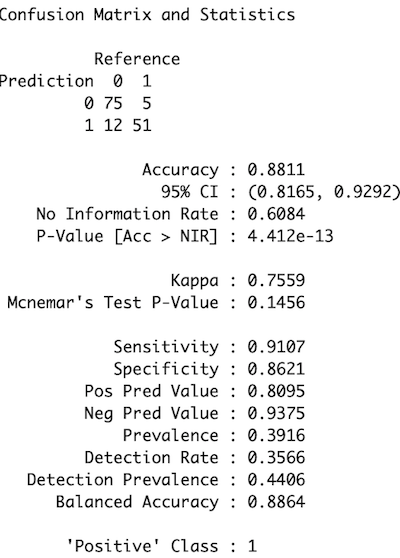
\includegraphics[width=0.9\textwidth]{ThesisTemplate/appendix/images/Chapter5Appendix/ConfusionMatrix75/BreastCancer.png}
        \caption{Confusion Matrix output for Random Forest fitted to the Breast Cancer Dataset after under-sampling (75\% majority class retained)}
        \label{fig:my_label}
    \end{minipage}
\end{figure}

\begin{figure}[!htbp]
    \centering
    \begin{minipage}{0.45\textwidth}
        \centering
        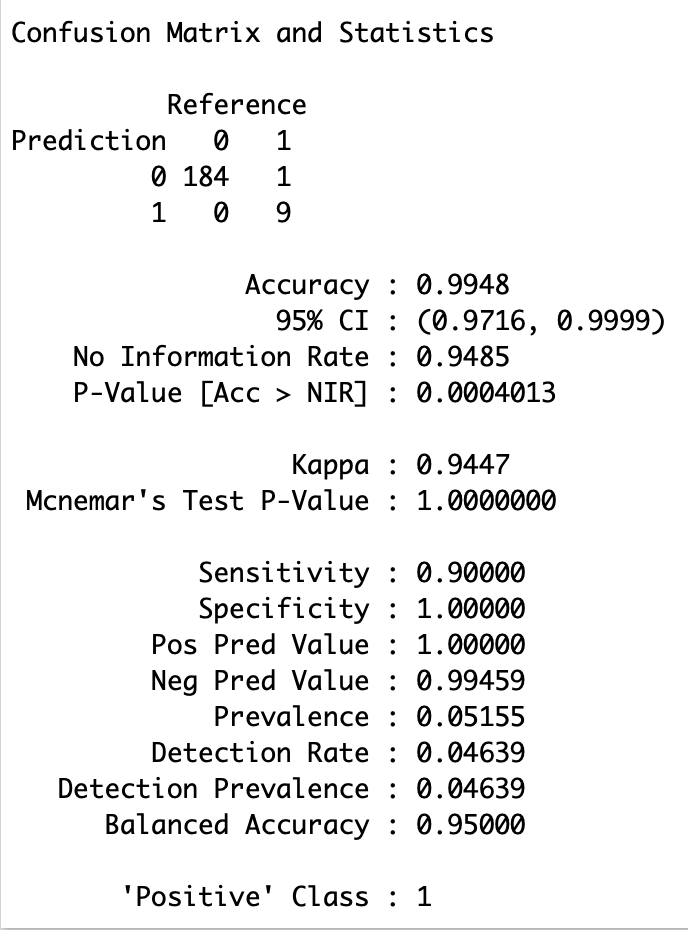
\includegraphics[width=0.9\textwidth]{ThesisTemplate/appendix/images/Chapter5Appendix/ConfusionMatrix75/CervicalCancer.png}
        \caption{Confusion Matrix output for Random Forest fitted to the Cervical Cancer Dataset after under-sampling (75\% majority class retained)}
        \label{fig:my_label}
    \end{minipage}\hfill
    \begin{minipage}{0.45\textwidth}
        \centering
        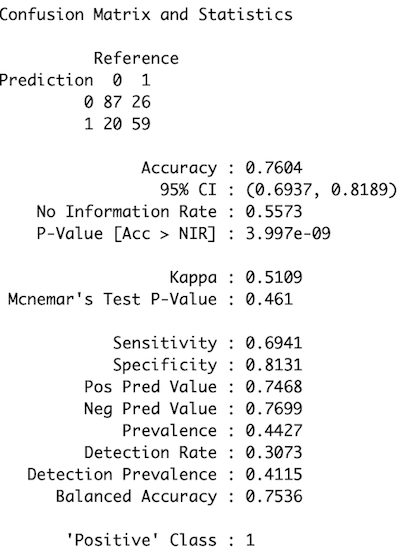
\includegraphics[width=0.9\textwidth]{ThesisTemplate/appendix/images/Chapter5Appendix/ConfusionMatrix75/Diabetes.png}
        \caption{Confusion Matrix output for Random Forest fitted to the Diabetes Dataset after under-sampling (75\% majority class retained)}
        \label{fig:my_label}
    \end{minipage}
\end{figure}

\begin{figure}[!htbp]
    \centering
    \begin{minipage}{0.45\textwidth}
        \centering
        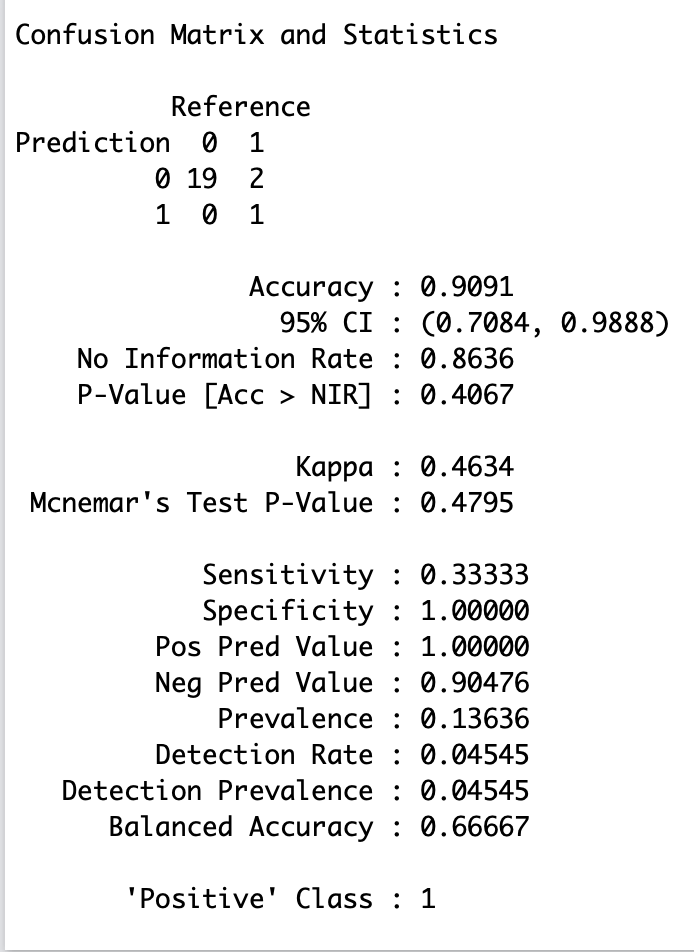
\includegraphics[width=0.9\textwidth]{ThesisTemplate/appendix/images/Chapter5Appendix/ConfusionMatrix75/Fertility.png}
        \caption{Confusion Matrix output for Random Forest fitted to the Fertility Dataset after under-sampling (75\% majority class retained)}
        \label{fig:my_label}
    \end{minipage}\hfill
    \begin{minipage}{0.45\textwidth}
        \centering
        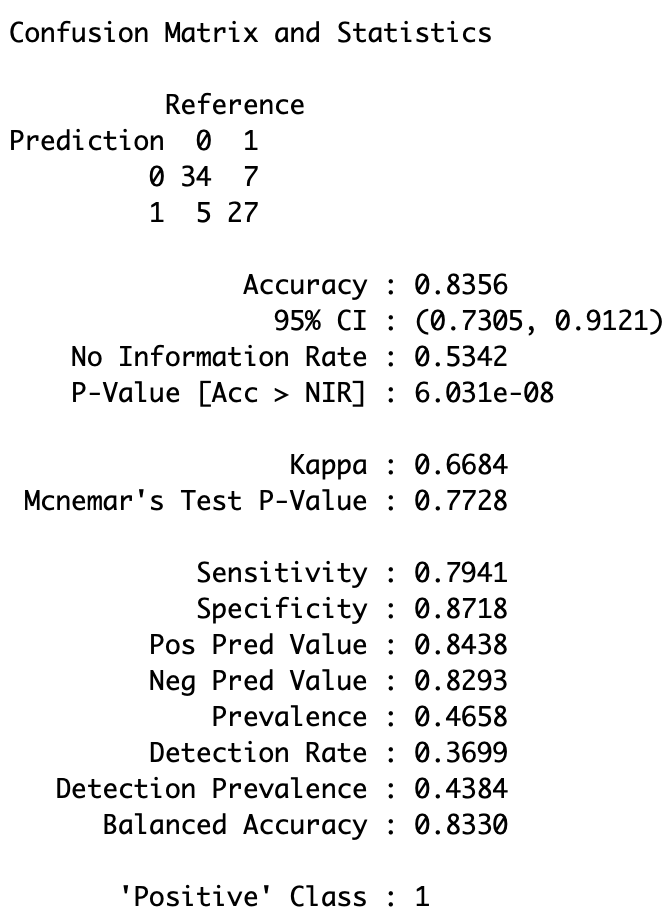
\includegraphics[width=0.9\textwidth]{ThesisTemplate/appendix/images/Chapter5Appendix/ConfusionMatrix75/HA.png}
        \caption{Confusion Matrix output for Random Forest fitted to the Heart Attack Dataset after under-sampling (75\% majority class retained)}
        \label{fig:my_label}
    \end{minipage}
\end{figure}

\begin{figure}[!htbp]
    \centering
    \begin{minipage}{0.45\textwidth}
        \centering
        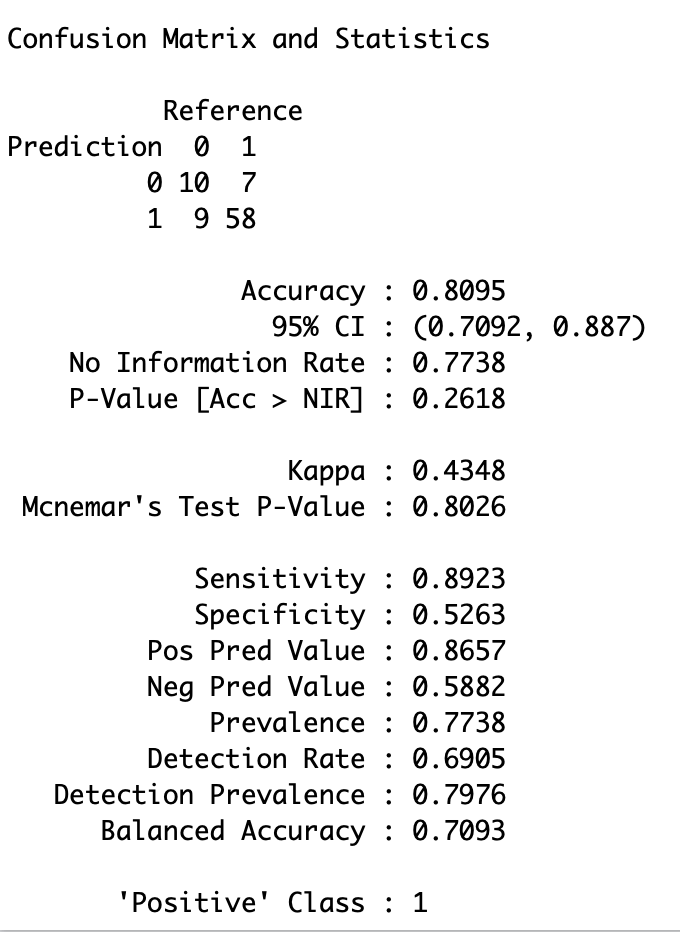
\includegraphics[width=0.9\textwidth]{ThesisTemplate/appendix/images/Chapter5Appendix/ConfusionMatrix75/LBP.png}
        \caption{Confusion Matrix output for Random Forest fitted to the Low Back Pain Dataset after under-sampling (75\% majority class retained)}
        \label{fig:my_label}
    \end{minipage}\hfill
    \begin{minipage}{0.45\textwidth}
        \centering
        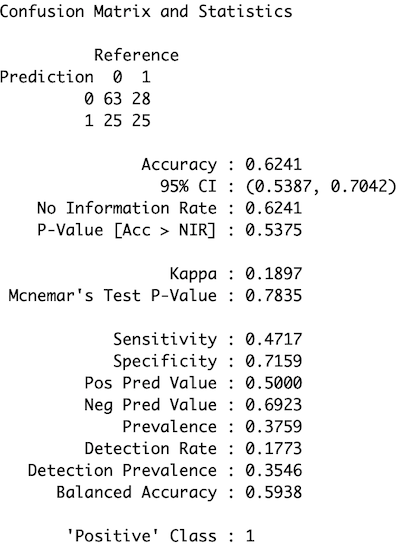
\includegraphics[width=0.9\textwidth]{ThesisTemplate/appendix/images/Chapter5Appendix/ConfusionMatrix75/Liver.png}
        \caption{Confusion Matrix output for Random Forest fitted to the Liver Dataset after under-sampling (75\% majority class retained)}
        \label{fig:my_label}
    \end{minipage}
\end{figure}

\begin{figure}[!htbp]
    \centering
    \begin{minipage}{0.45\textwidth}
        \centering
        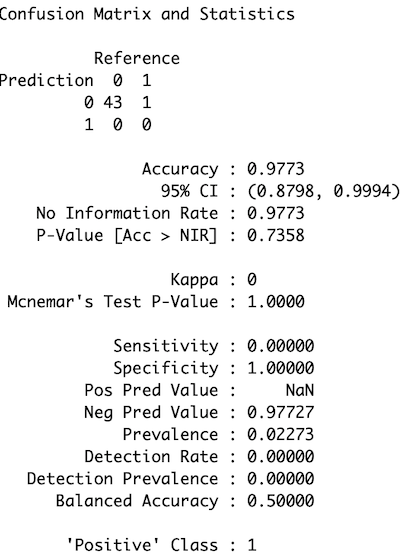
\includegraphics[width=0.9\textwidth]{ThesisTemplate/appendix/images/Chapter5Appendix/ConfusionMatrix75/ModifiedHA.png}
        \caption{Confusion Matrix output for Random Forest fitted to the Modified Heart Attack Dataset after under-sampling (75\% majority class retained)}
        \label{fig:my_label}
    \end{minipage}\hfill
    \begin{minipage}{0.45\textwidth}
        \centering
        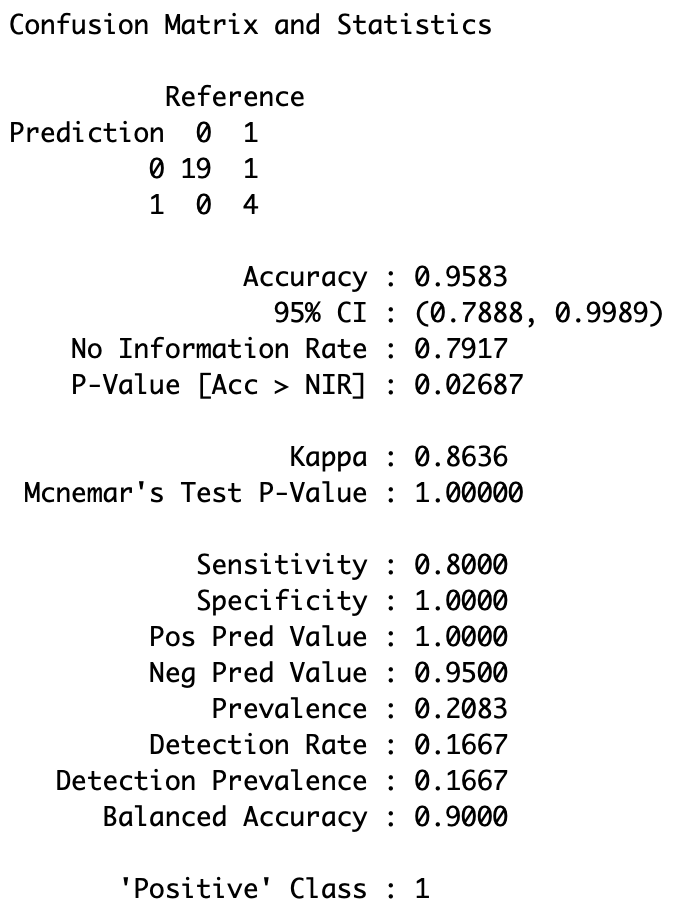
\includegraphics[width=0.9\textwidth]{ThesisTemplate/appendix/images/Chapter5Appendix/ConfusionMatrix75/ModifiedLBP.png}
        \caption{Confusion Matrix output for Random Forest fitted to the Modified Low Back Pain Dataset after under-sampling (75\% majority class retained)}
        \label{fig:my_label}
    \end{minipage}
\end{figure}

\begin{figure}[!htbp]
    \centering
    \begin{minipage}{0.45\textwidth}
        \centering
        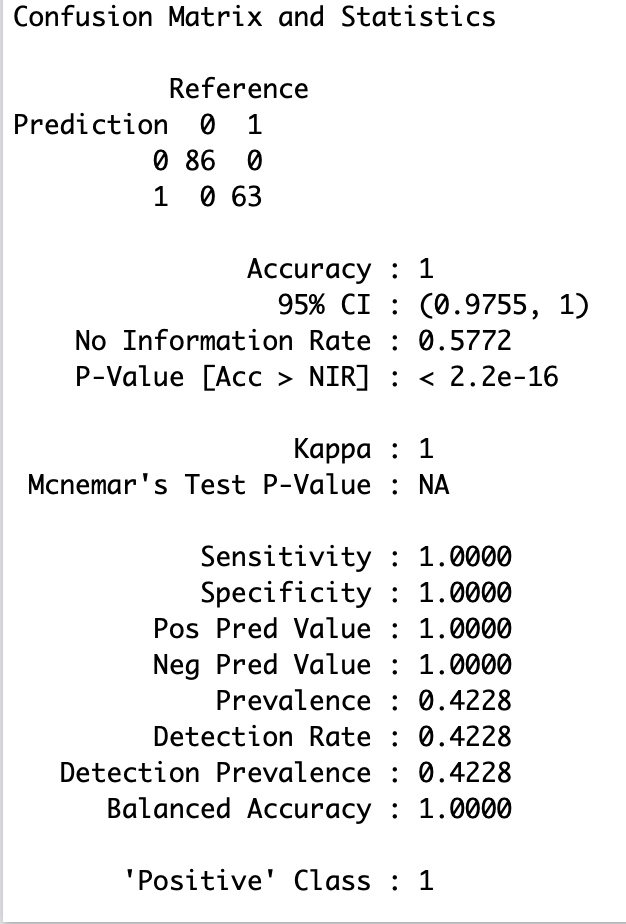
\includegraphics[width=0.9\textwidth]{ThesisTemplate/appendix/images/Chapter5Appendix/ConfusionMatrix60/Autism.png}
        \caption{Confusion Matrix output for Random Forest fitted to the Autism Dataset after under-sampling (60\% majority class retained)}
        \label{fig:my_label}
    \end{minipage}\hfill
    \begin{minipage}{0.45\textwidth}
        \centering
        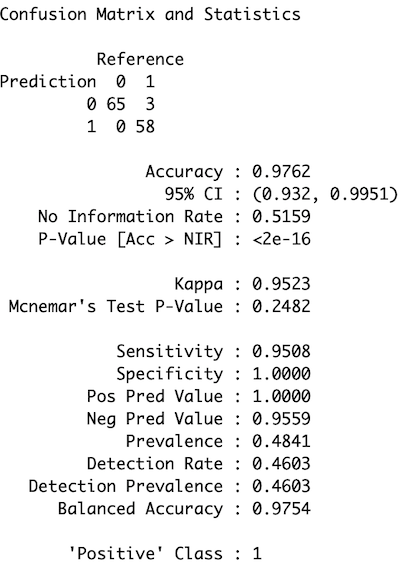
\includegraphics[width=0.9\textwidth]{ThesisTemplate/appendix/images/Chapter5Appendix/ConfusionMatrix60/BreastCancer.png}
        \caption{Confusion Matrix output for Random Forest fitted to the Breast Cancer Dataset after under-sampling (60\% majority class retained)}
        \label{fig:my_label}
    \end{minipage}
\end{figure}

\begin{figure}[!htbp]
    \centering
    \begin{minipage}{0.45\textwidth}
        \centering
        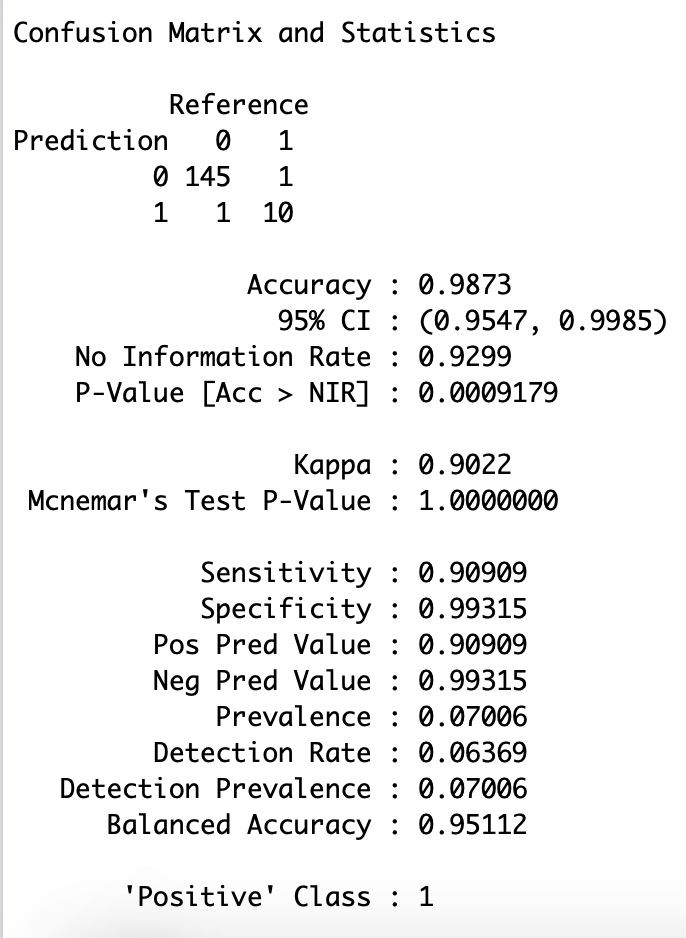
\includegraphics[width=0.9\textwidth]{ThesisTemplate/appendix/images/Chapter5Appendix/ConfusionMatrix60/CervicalCancer.png}
        \caption{Confusion Matrix output for Random Forest fitted to the Cervical Cancer after under-sampling (60\% majority class retained)}
        \label{fig:my_label}
    \end{minipage}\hfill
    \begin{minipage}{0.45\textwidth}
        \centering
        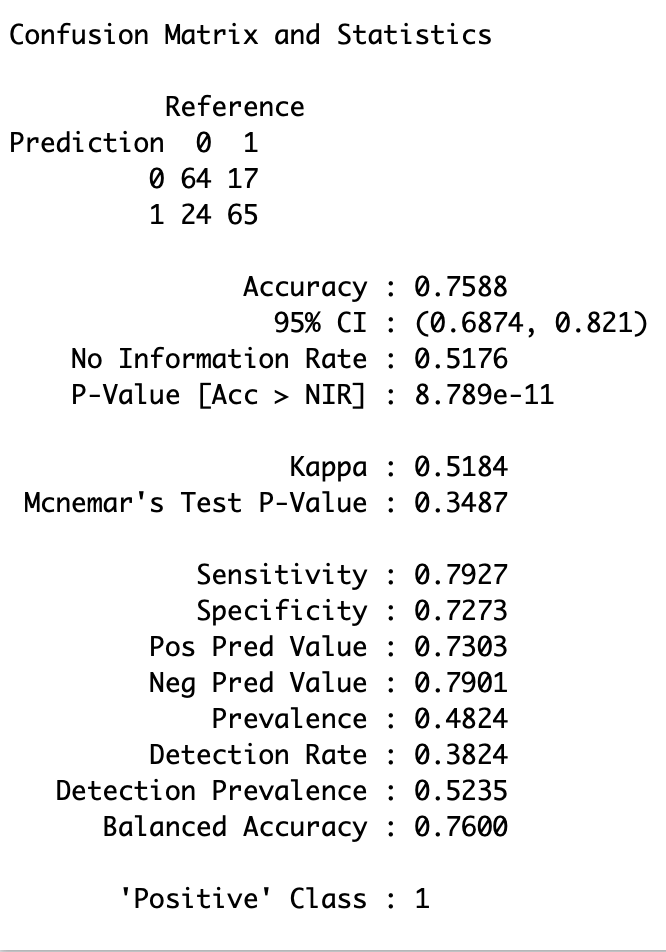
\includegraphics[width=0.9\textwidth]{ThesisTemplate/appendix/images/Chapter5Appendix/ConfusionMatrix60/Diabetes.png}
        \caption{Confusion Matrix output for Random Forest fitted to the Diabetes Dataset after under-sampling (60\% majority class retained)}
        \label{fig:my_label}
    \end{minipage}
\end{figure}

\begin{figure}[!htbp]
    \centering
    \begin{minipage}{0.45\textwidth}
        \centering
        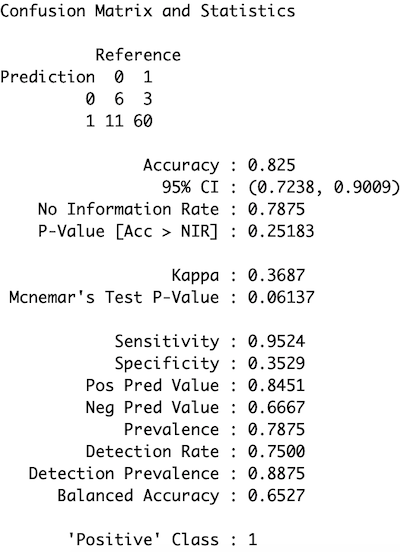
\includegraphics[width=0.9\textwidth]{ThesisTemplate/appendix/images/Chapter5Appendix/ConfusionMatrix60/LBP.png}
        \caption{Confusion Matrix output for Random Forest fitted to the Low Back Pain Dataset after under-sampling (60\% majority class retained)}
        \label{fig:my_label}
    \end{minipage}\hfill
    \begin{minipage}{0.45\textwidth}
        \centering
        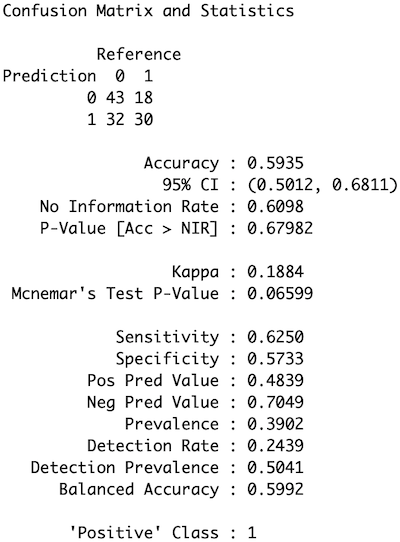
\includegraphics[width=0.9\textwidth]{ThesisTemplate/appendix/images/Chapter5Appendix/ConfusionMatrix60/Liver.png}
        \caption{Confusion Matrix output for Random Forest fitted to the Liver Dataset after under-sampling (60\% majority class retained)}
        \label{fig:my_label}
    \end{minipage}
\end{figure}

\begin{figure}[!htbp]
    \centering
    \begin{minipage}{0.45\textwidth}
        \centering
        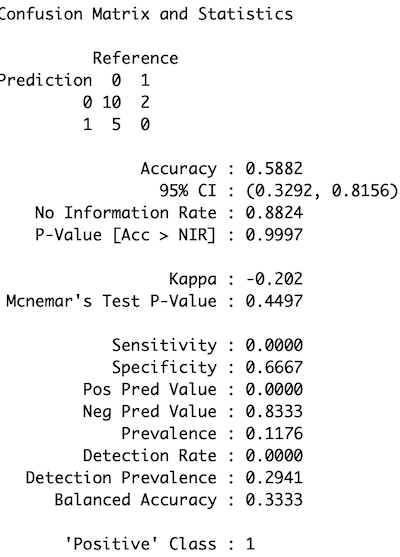
\includegraphics[width=0.9\textwidth]{ThesisTemplate/appendix/images/Chapter5Appendix/ConfusionMatrix60/Fertility.png}
        \caption{Confusion Matrix output for Random Forest fitted to the Fertility Dataset after under-sampling (60\% majority class retained)}
        \label{fig:my_label}
    \end{minipage}\hfill
    \begin{minipage}{0.45\textwidth}
        \centering
        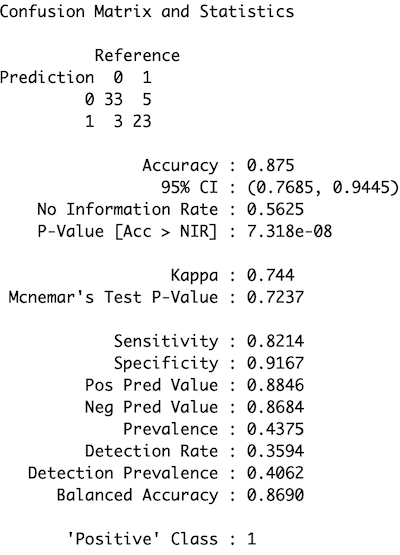
\includegraphics[width=0.9\textwidth]{ThesisTemplate/appendix/images/Chapter5Appendix/ConfusionMatrix60/HA.png}
        \caption{Confusion Matrix output for Random Forest fitted to the Heart Attack Dataset after under-sampling (60\% majority class retained)}
        \label{fig:my_label}
    \end{minipage}
\end{figure}

\begin{figure}[!htbp]
    \centering
    \begin{minipage}{0.45\textwidth}
        \centering
        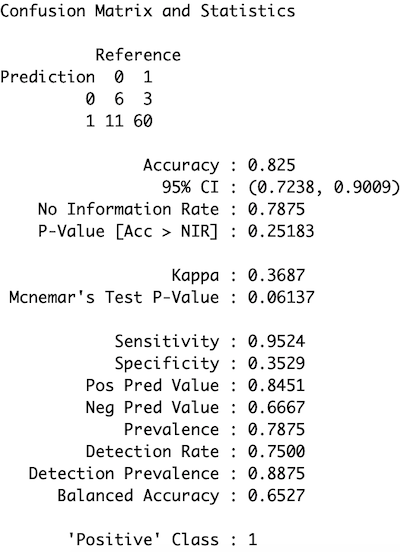
\includegraphics[width=0.9\textwidth]{ThesisTemplate/appendix/images/Chapter5Appendix/ConfusionMatrix60/LBP.png}
        \caption{Confusion Matrix output for Random Forest fitted to the Low Back Pain Dataset after under-sampling (60\% majority class retained)}
        \label{fig:my_label}
    \end{minipage}\hfill
    \begin{minipage}{0.45\textwidth}
        \centering
        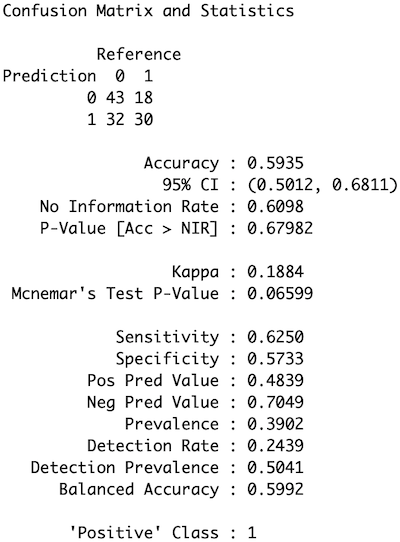
\includegraphics[width=0.9\textwidth]{ThesisTemplate/appendix/images/Chapter5Appendix/ConfusionMatrix60/Liver.png}
        \caption{Confusion Matrix output for Random Forest fitted to the Liver Dataset after under-sampling (60\% majority class retained)}
        \label{fig:my_label}
    \end{minipage}
\end{figure}

\begin{figure}[!htbp]
    \centering
    \begin{minipage}{0.45\textwidth}
        \centering
        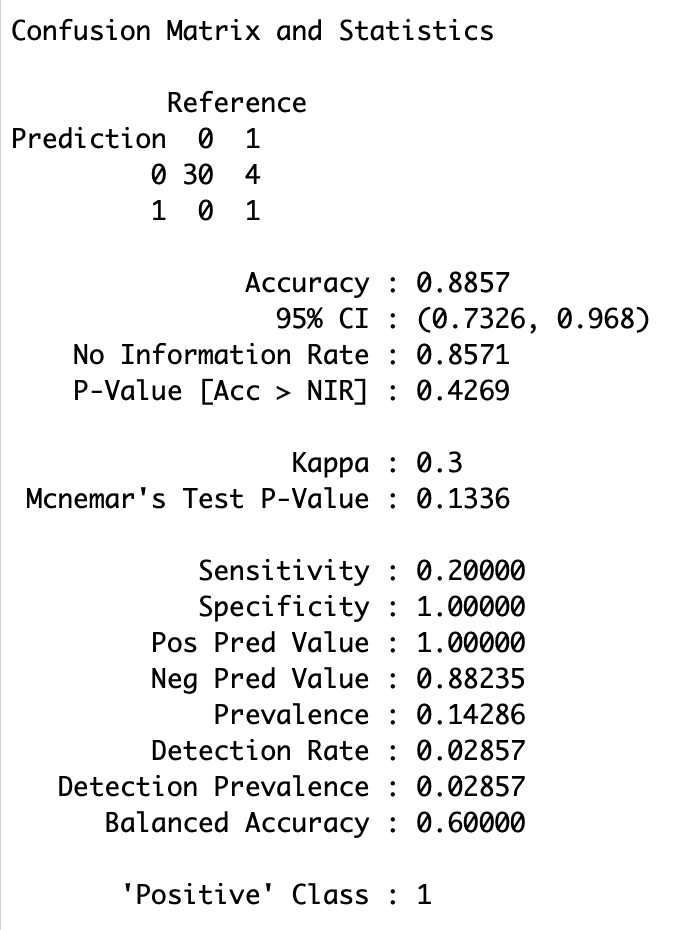
\includegraphics[width=0.9\textwidth]{ThesisTemplate/appendix/images/Chapter5Appendix/ConfusionMatrix60/modHA.png}
        \caption{Confusion Matrix output for Random Forest fitted to the Modified Heart Attack Dataset after under-sampling (60\% majority class retained)}
        \label{fig:my_label}
    \end{minipage}\hfill
    \begin{minipage}{0.45\textwidth}
        \centering
        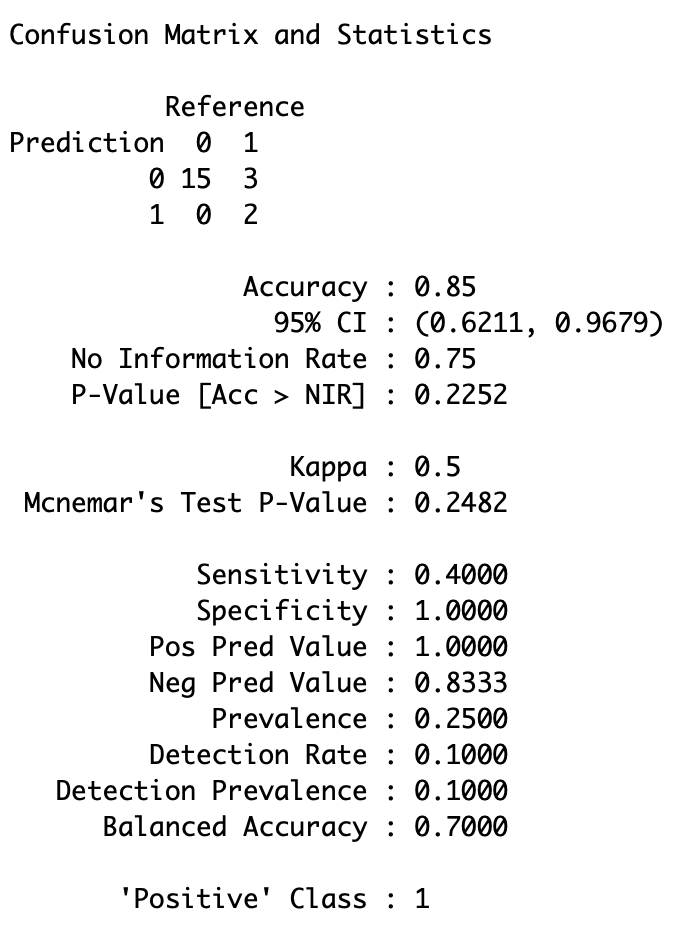
\includegraphics[width=0.9\textwidth]{ThesisTemplate/appendix/images/Chapter5Appendix/ConfusionMatrix60/modLBP.png}
        \caption{Confusion Matrix output for Random Forest fitted to the Modified Low Back Pain Dataset after under-sampling (60\% majority class retained)}
        \label{fig:my_label}
    \end{minipage}
\end{figure}

\begin{figure}[!htbp]
    \centering
    \begin{minipage}{0.45\textwidth}
        \centering
        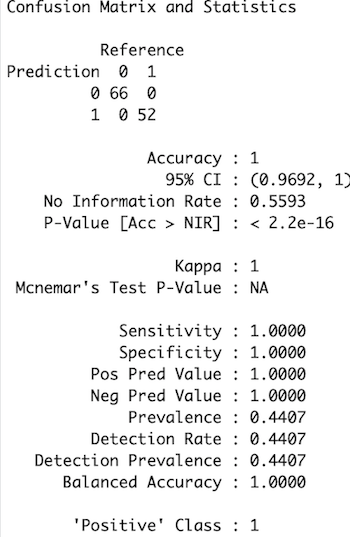
\includegraphics[width=0.9\textwidth]{ThesisTemplate/appendix/images/Chapter5Appendix/ConfusionMatrix40/Autism.png}
        \caption{Confusion Matrix output for Random Forest fitted to the Autism Dataset after under-sampling (40\% majority class retained)}
        \label{fig:my_label}
    \end{minipage}\hfill
    \begin{minipage}{0.45\textwidth}
        \centering
        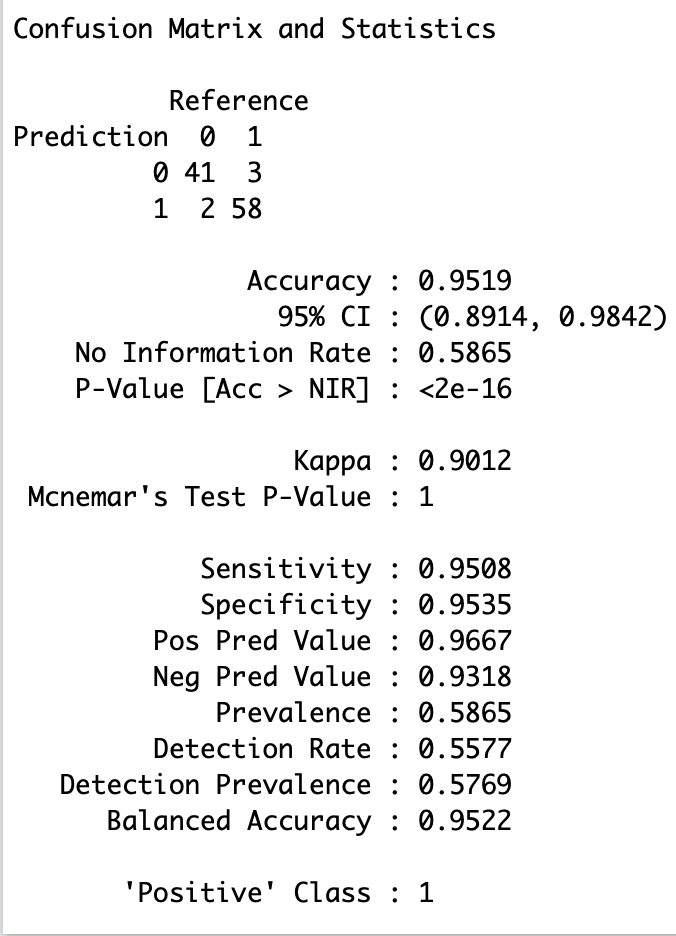
\includegraphics[width=0.9\textwidth]{ThesisTemplate/appendix/images/Chapter5Appendix/ConfusionMatrix40/BreastCancer.png}
        \caption{Confusion Matrix output for Random Forest fitted to the Breast Cancer Dataset after under-sampling (40\% majority class retained)}
        \label{fig:my_label}
    \end{minipage}
\end{figure}

\begin{figure}[!htbp]
    \centering
    \begin{minipage}{0.45\textwidth}
        \centering
        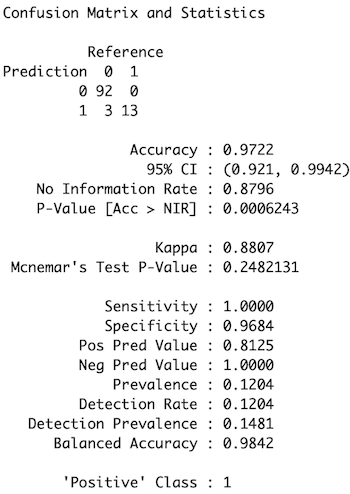
\includegraphics[width=0.9\textwidth]{ThesisTemplate/appendix/images/Chapter5Appendix/ConfusionMatrix40/CervicalCancer.png}
        \caption{Confusion Matrix output for Random Forest fitted to the Cervical Cancer Dataset after under-sampling (40\% majority class retained)}
        \label{fig:my_label}
    \end{minipage}\hfill
    \begin{minipage}{0.45\textwidth}
        \centering
        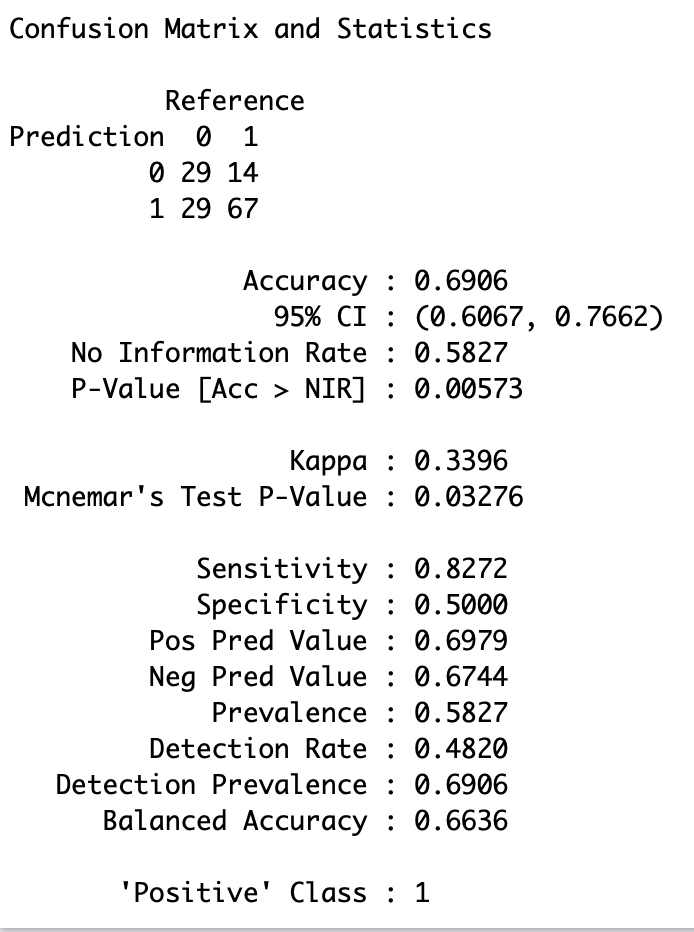
\includegraphics[width=0.9\textwidth]{ThesisTemplate/appendix/images/Chapter5Appendix/ConfusionMatrix40/Diabetes.png}
        \caption{Confusion Matrix output for Random Forest fitted to the Diabetes Dataset after under-sampling (40\% majority class retained)}
        \label{fig:my_label}
    \end{minipage}
\end{figure}

\begin{figure}[!htbp]
    \centering
    \begin{minipage}{0.45\textwidth}
        \centering
        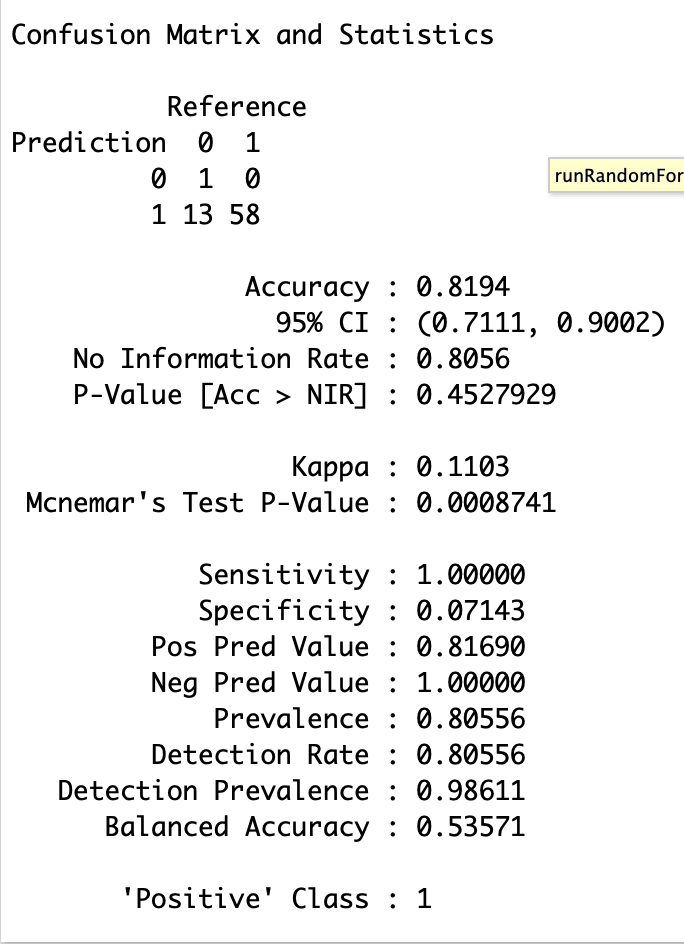
\includegraphics[width=0.9\textwidth]{ThesisTemplate/appendix/images/Chapter5Appendix/ConfusionMatrix40/LBP.png}
        \caption{Confusion Matrix output for Random Forest fitted to the Low Back Pain Dataset after under-sampling (40\% majority class retained)}
        \label{fig:my_label}
    \end{minipage}\hfill
    \begin{minipage}{0.45\textwidth}
        \centering
        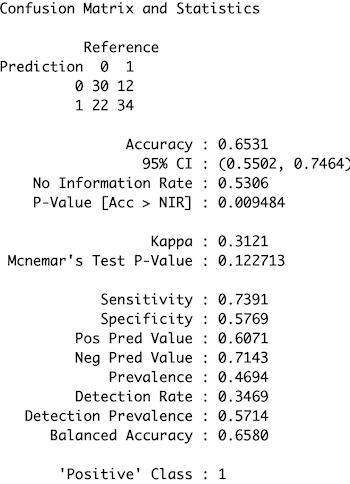
\includegraphics[width=0.9\textwidth]{ThesisTemplate/appendix/images/Chapter5Appendix/ConfusionMatrix40/Liver.png}
        \caption{Confusion Matrix output for Random Forest fitted to the Liver Dataset after under-sampling (40\% majority class retained)}
        \label{fig:my_label}
    \end{minipage}
\end{figure}

\begin{figure}[!htbp]
    \centering
    \begin{minipage}{0.45\textwidth}
        \centering
        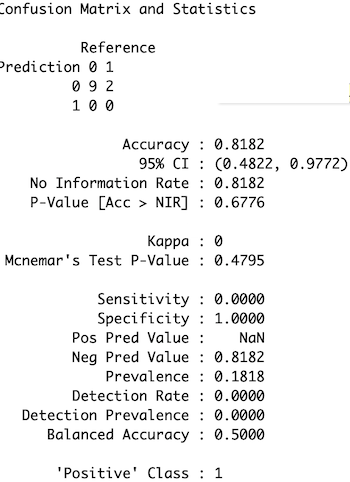
\includegraphics[width=0.9\textwidth]{ThesisTemplate/appendix/images/Chapter5Appendix/ConfusionMatrix40/Fertility.png}
        \caption{Confusion Matrix output for Random Forest fitted to the Fertility Dataset after under-sampling (40\% majority class retained)}
        \label{fig:my_label}
    \end{minipage}\hfill
    \begin{minipage}{0.45\textwidth}
        \centering
        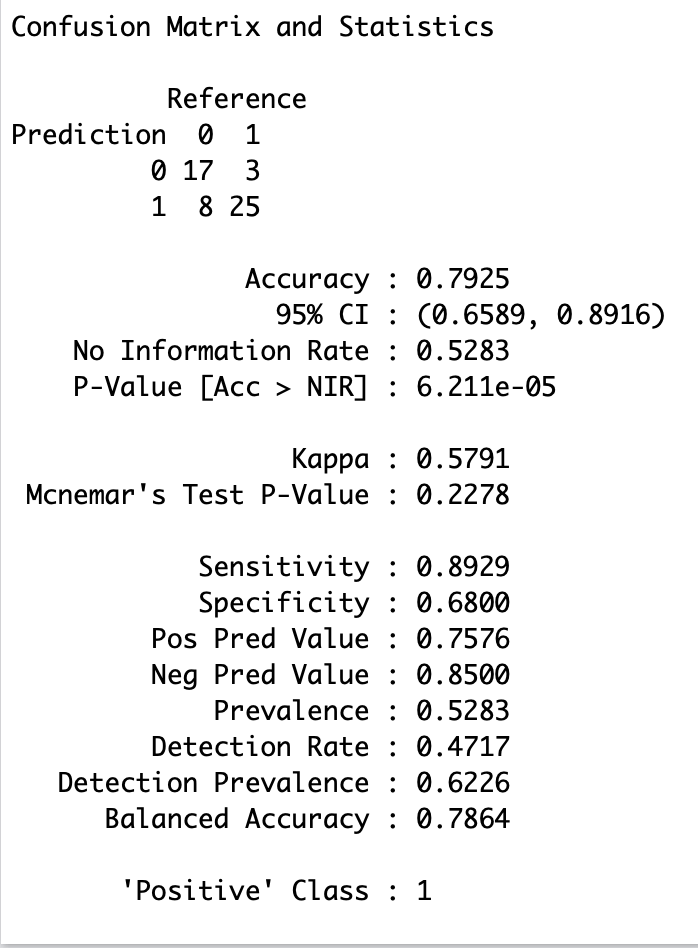
\includegraphics[width=0.9\textwidth]{ThesisTemplate/appendix/images/Chapter5Appendix/ConfusionMatrix40/HA.png}
        \caption{Confusion Matrix output for Random Forest fitted to the Heart Attack Dataset after under-sampling (40\% majority class retained)}
        \label{fig:my_label}
    \end{minipage}
\end{figure}


\begin{figure}[!htbp]
    \centering
    \begin{minipage}{0.45\textwidth}
        \centering
        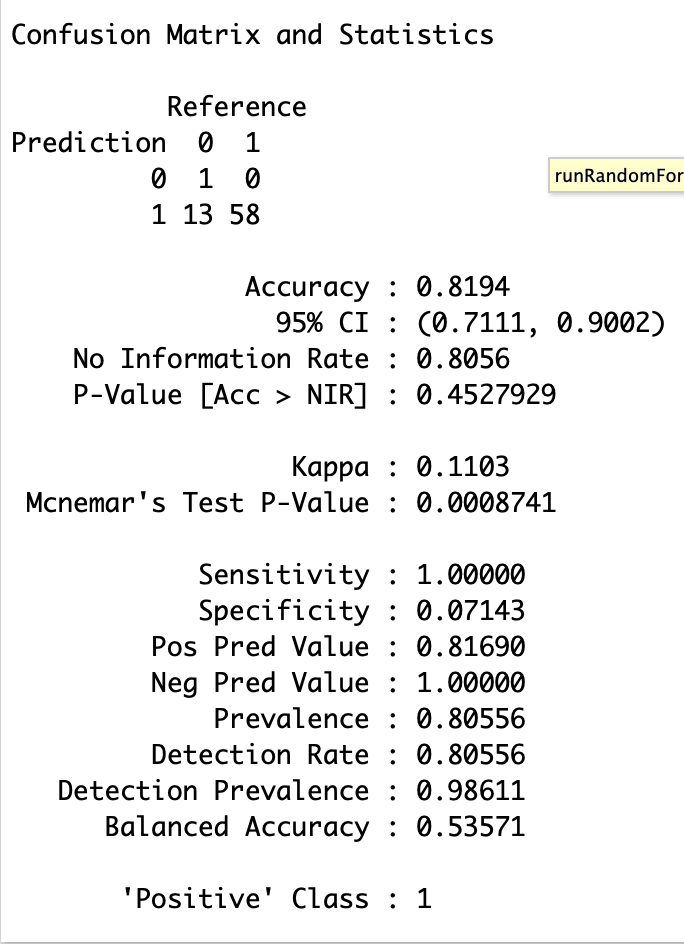
\includegraphics[width=0.9\textwidth]{ThesisTemplate/appendix/images/Chapter5Appendix/ConfusionMatrix40/LBP.png}
        \caption{Confusion Matrix output for Random Forest fitted to the Low Back Pain Dataset after under-sampling (40\% majority class retained)}
        \label{fig:my_label}
    \end{minipage}\hfill
    \begin{minipage}{0.45\textwidth}
        \centering
        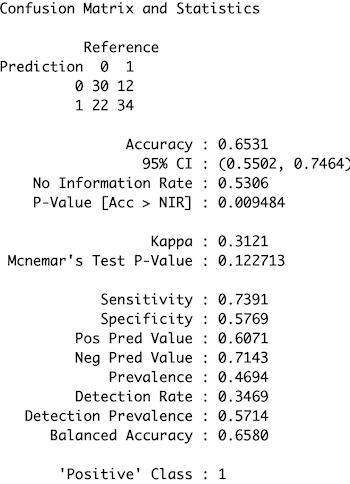
\includegraphics[width=0.9\textwidth]{ThesisTemplate/appendix/images/Chapter5Appendix/ConfusionMatrix40/Liver.png}
        \caption{Confusion Matrix output for Random Forest fitted to the Liver Dataset after under-sampling (40\% majority class retained)}
        \label{fig:my_label}
    \end{minipage}
\end{figure}

\begin{figure}[!htbp]
    \centering
    \begin{minipage}{0.45\textwidth}
        \centering
        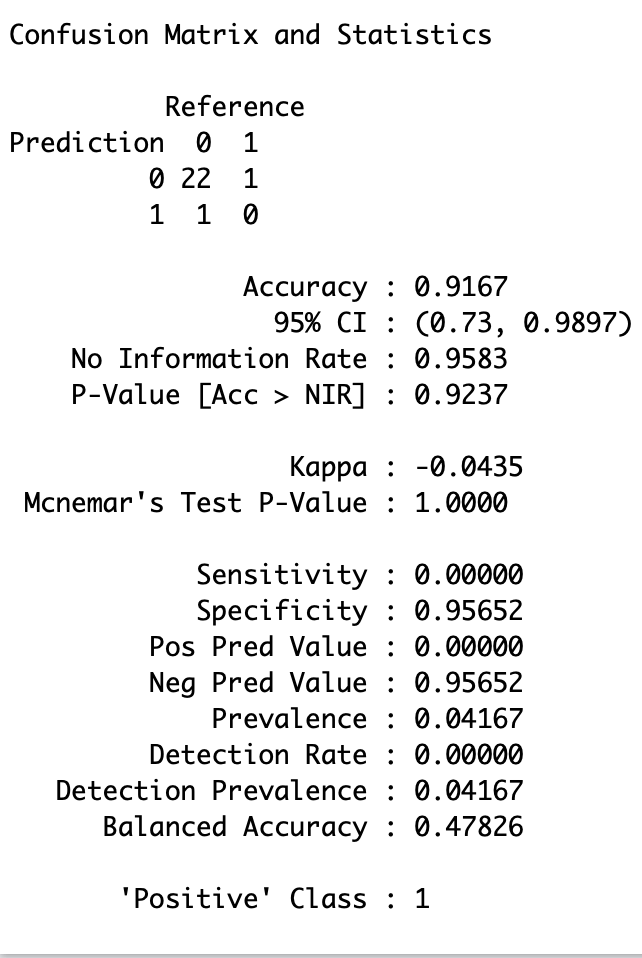
\includegraphics[width=0.9\textwidth]{ThesisTemplate/appendix/images/Chapter5Appendix/ConfusionMatrix40/modHA.png}
        \caption{Confusion Matrix output for Random Forest fitted to the Modified Heart Attack Dataset after under-sampling (40\% majority class retained)}
        \label{fig:my_label}
    \end{minipage}\hfill
    \begin{minipage}{0.45\textwidth}
        \centering
        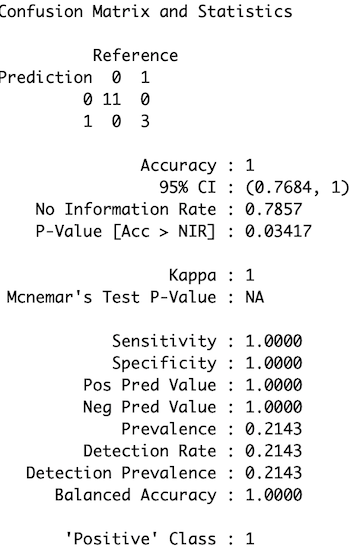
\includegraphics[width=0.9\textwidth]{ThesisTemplate/appendix/images/Chapter5Appendix/ConfusionMatrix40/modLBP.png}
        \caption{Confusion Matrix output for Random Forest fitted to the Modified Low Back Pain Dataset after under-sampling (40\% majority class retained)}
        \label{fig:my_label}
    \end{minipage}
\end{figure}


\begin{table}[ht]
\centering
\begin{tabular}{lrrr}
  \hline
  \rowcolor{LightCyan}
Dataset & Variation75 & Variation60 & Variation40 \\ 
  \hline
AuSDf & 0.00 & 0.00 & 0.00 \\ 
  BCDf & -0.04 & 0.06 & 0.04 \\ 
  CCDf & -0.00 & -0.01 & -0.02 \\ 
  DiabetesDf & 0.02 & 0.02 & -0.05 \\ 
  FertDf & -0.02 & -0.34 & -0.11 \\ 
  HAPDf & -0.07 & -0.03 & -0.12 \\ 
  LBPDf & -0.01 & 0.01 & 0.00 \\ 
  LiverDf & -0.09 & -0.12 & -0.06 \\ 
  subHAPDf & 0.03 & -0.06 & -0.03 \\ 
  subLBPDf & 0.05 & -0.06 & 0.09 \\ 
   \hline
\end{tabular}
\caption{Observed variations in accuracy for all datasets for the three different conditions of under-sampling}
\end{table}

\begin{table}[ht]
\centering
\begin{tabular}{lrrr}
  \hline
   \rowcolor{LightCyan}
Dataset & Variation75 & Variation60 & Variation40 \\ 
  \hline
AuSDf & 0.00 & 0.00 & 0.00 \\ 
  BCDf & 0.06 & 0.10 & 0.10 \\ 
  CCDf & 0.00 & 0.01 & 0.10 \\ 
  DiabetesDf & 0.14 & 0.24 & 0.27 \\ 
  FertDf & 0.33 & 0.00 & 0.00 \\ 
  HAPDf & -0.04 & -0.01 & 0.06 \\ 
  LBPDf & -0.01 & 0.05 & 0.10 \\ 
  LiverDf & 0.12 & 0.27 & 0.39 \\ 
  subHAPDf & 0.00 & 0.20 & 0.00 \\ 
  subLBPDf & 0.30 & -0.10 & 0.50 \\ 
   \hline
\end{tabular}
\caption{Observed variations in sensitivity for all datasets for the three different conditions of under-sampling}
\end{table}

\begin{table}[ht]
\centering
\begin{tabular}{lrrr}
  \hline
  \rowcolor{LightCyan}
Dataset & Variation75 & Variation60 & Variation40 \\ 
  \hline
AuSDf & 0.00 & 0.00 & 0.00 \\ 
  BCDf & -0.13 & 0.06 & 0.03 \\ 
  CCDf & 0.00 & -0.09 & -0.19 \\ 
  DiabetesDf & 0.02 & 0.01 & -0.03 \\ 
  FertDf &  &  &  \\ 
  HAPDf & -0.05 & -0.01 & -0.14 \\ 
  LBPDf & 0.03 & 0.01 & -0.02 \\ 
  LiverDf & -0.08 & -0.09 & 0.03 \\ 
  subHAPDf &  & 1.00 & 0.00 \\ 
  subLBPDf & 0.00 & 0.00 & 0.00 \\ 
   \hline
\end{tabular}
\caption{Observed variations in precision for all datasets for the three different conditions of under-sampling}
\end{table}

\begin{table}[ht]
\centering
\begin{tabular}{lrrr}
  \hline
  \rowcolor{LightCyan}
Dataset & Variation75 & Variation60 & Variation40 \\ 
  \hline
AuSDf & 0.00 & 0.00 & 0.00 \\ 
  BCDf & -0.04 & 0.08 & 0.06 \\ 
  CCDf & 0.00 & -0.04 & -0.05 \\ 
  DiabetesDf & 0.09 & 0.13 & 0.13 \\ 
  FertDf &  &  &  \\ 
  HAPDf & -0.04 & -0.01 & -0.04 \\ 
  LBPDf & 0.01 & 0.03 & 0.03 \\ 
  LiverDf & 0.05 & 0.11 & 0.23 \\ 
  subHAPDf &  &  &  \\ 
  subLBPDf & 0.22 & -0.10 & 0.33 \\ 
   \hline
\end{tabular}
\caption{Observed variations in F1 score for all datasets for the three different conditions of under-sampling}
\end{table}



 

\chapter{Project Log}







